\section{CI/CD Chain} % A complete description of stages and tools included in the CI/CD chains, including deployment and release of your systems.

In order to introduce continous integration and continous deployment to the program, we used github actions, namely workflows. The project included several different workflows as described in table \ref{tab:workflows}. Furthermore, the workflows work together, and in order to capture the experience as a developer working on this project and the conditions for the different workflows to run see figure \ref{fig:workflows}.

\begin{table}[]
    \centering
    \begin{tabular}{l|l}
        \textbf{Workflow file} & \textbf{Function}\\
        \hline
        \textit{AutomaticBuildRelease.Backend} &  Bumps the patch versioning of the \textit{MinitwitSimulatorAPI} project and creates a release on the github repository.\\
        \textit{AutomaticBuildRelease.Frontend} & Bumps the patch versioning of the \textit{Minitwit} project and creates a release on the github repository.\\
        \textit{WeeklyMinorRelease} & Bumps the minor version of the entire program and creates a release each Thursday at 20:00 UTC.\\
        \textit{Linters-and\_Formatter} & Runs hadolint, precommit, and the dotnet-format linter, when a PR is created, modified, and reopened.\\
        \textit{Testing} & Runs all tests on the infrastructure, the frontend, and the backend, when a PR is created, modified, and reopened.\\
        \textit{Provision-and-Deploy} & Provision and deploy swarm and observability servers using ansible for server provision and pulumi for infrastructure as code, on pushes to main.\\
        \textit{latex-build} & Creates a report PDF, when changes have been made to the report.
    \end{tabular}
    \caption{The function of the workflows}
    \label{tab:workflows}
\end{table}

The conditions for the workflows being run can be seen in figure \ref{fig:workflows}.

\begin{figure}
    \centering
    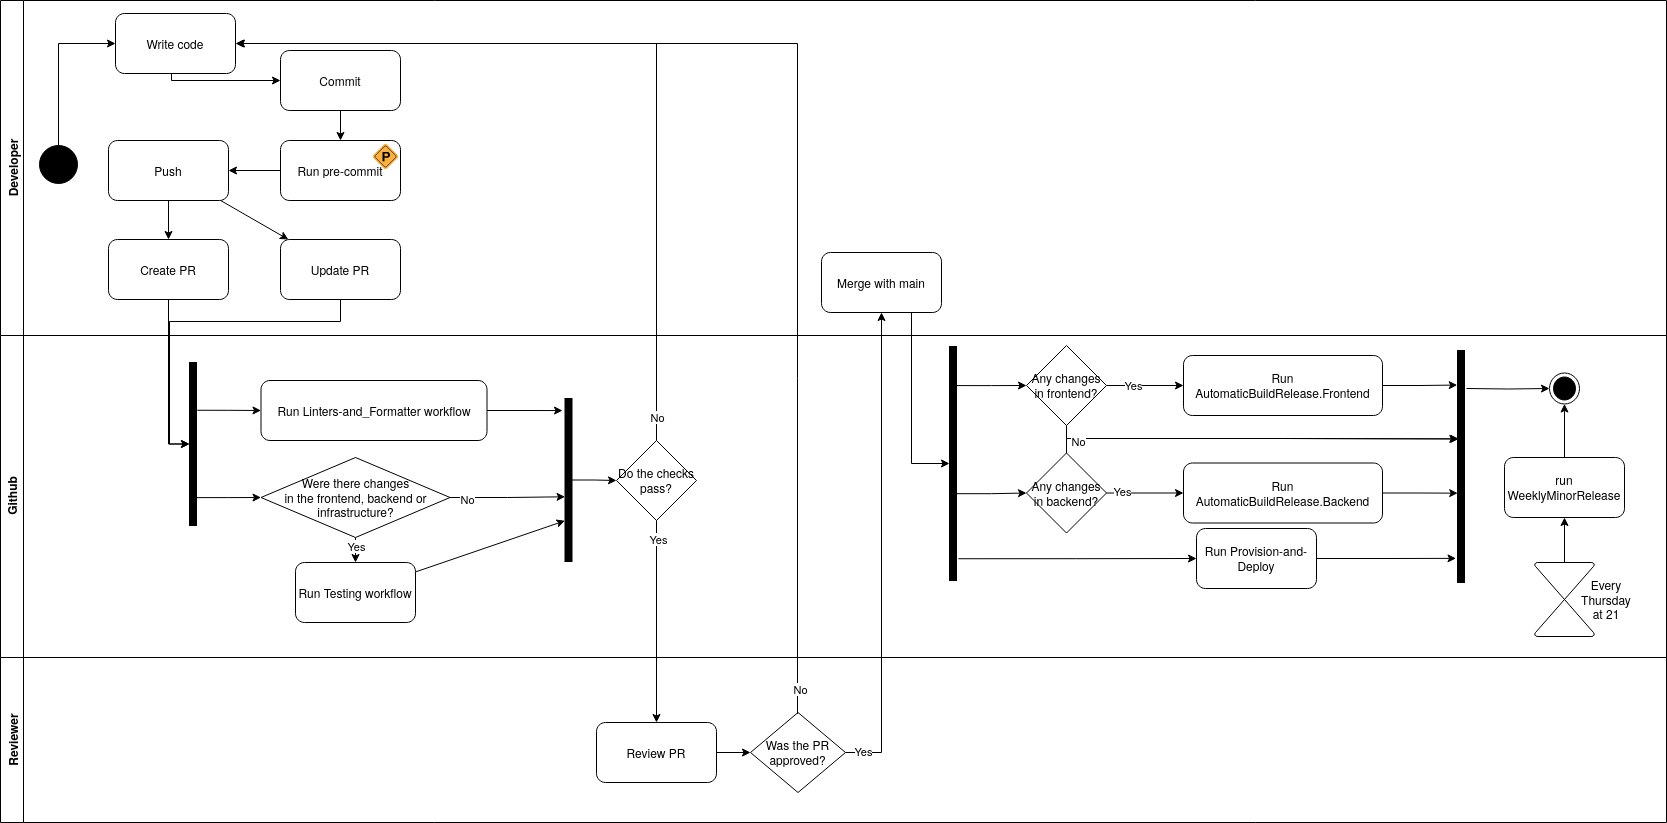
\includegraphics{report/images/Github-Actions.png}
    \caption{Activity diagram showcasing the workflows interacting }
    \label{fig:workflows}
\end{figure}

